\documentclass[tikz,border=8pt]{standalone}
\usepackage{amsmath}
\usetikzlibrary{arrows.meta,positioning,fit}

\begin{document}
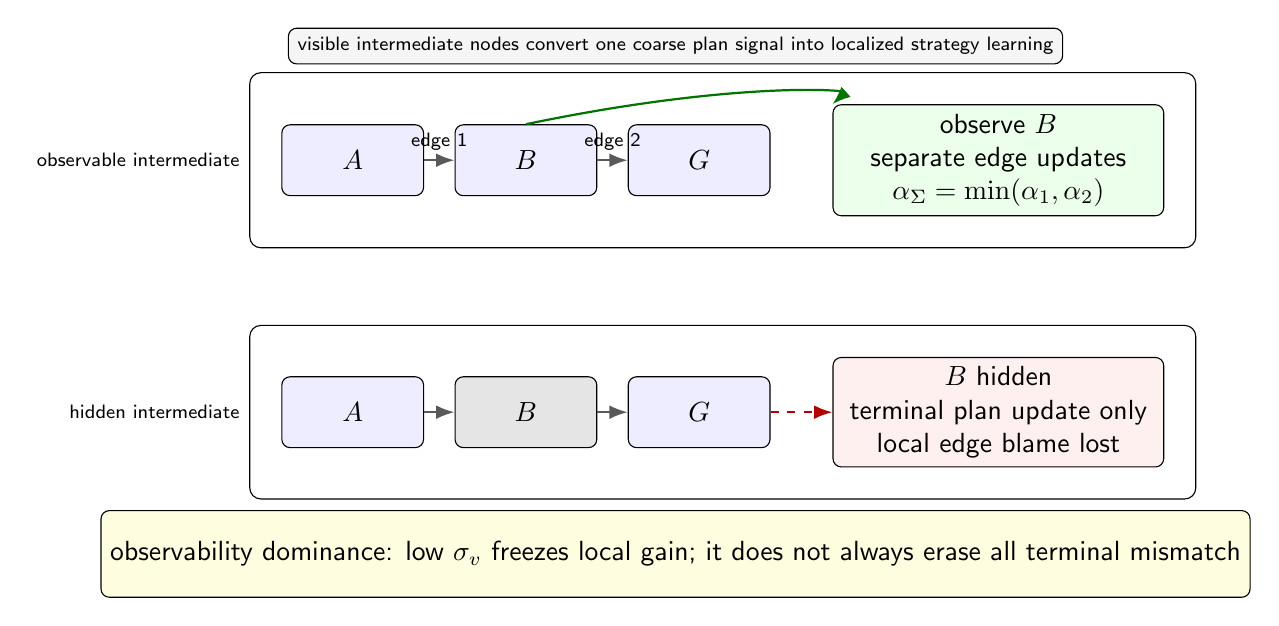
\begin{tikzpicture}[
  font=\sffamily,
  nodebox/.style={draw, rounded corners=3pt, align=center, minimum width=18mm, minimum height=9mm, fill=white},
  box/.style={draw, rounded corners=3pt, align=center, minimum width=42mm, minimum height=11mm, fill=white},
  note/.style={align=center, font=\sffamily\scriptsize},
  arrow/.style={-Latex, thick, draw=black!65},
  good/.style={-Latex, thick, draw=green!45!black},
  bad/.style={-Latex, thick, dashed, draw=red!70!black}
]

\node[nodebox, fill=blue!7] (a1) at (0,2) {$A$};
\node[nodebox, fill=blue!7] (b1) at (2.2,2) {$B$};
\node[nodebox, fill=blue!7] (g1) at (4.4,2) {$G$};
\draw[arrow] (a1) -- node[above, note] {edge 1} (b1);
\draw[arrow] (b1) -- node[above, note] {edge 2} (g1);
\node[box, fill=green!8] (obs1) at (8.2,2)
  {observe $B$\\separate edge updates\\$\alpha_\Sigma=\min(\alpha_1,\alpha_2)$};
\draw[good] (b1.north) .. controls (4.8,3.0) and (6.3,2.9) .. (obs1.north west);

\node[nodebox, fill=blue!7] (a2) at (0,-1.2) {$A$};
\node[nodebox, fill=gray!20] (b2) at (2.2,-1.2) {$B$};
\node[nodebox, fill=blue!7] (g2) at (4.4,-1.2) {$G$};
\draw[arrow] (a2) -- (b2);
\draw[arrow] (b2) -- (g2);
\node[box, fill=red!6] (obs2) at (8.2,-1.2)
  {$B$ hidden\\terminal plan update only\\local edge blame lost};
\draw[bad] (g2.east) -- (obs2.west);

\node[box, fill=yellow!12, minimum width=78mm] at (4.1,-3.0)
  {observability dominance: low $\sigma_v$ freezes local gain; it does not always erase all terminal mismatch};

\node[note, fill=gray!8, draw, rounded corners=3pt, minimum width=88mm] at (4.1,3.45)
  {visible intermediate nodes convert one coarse plan signal into localized strategy learning};

\node[draw, rounded corners=4pt, fit=(a1)(g1)(obs1), inner sep=4mm,
  label={[note]left:observable intermediate}] {};
\node[draw, rounded corners=4pt, fit=(a2)(g2)(obs2), inner sep=4mm,
  label={[note]left:hidden intermediate}] {};

\end{tikzpicture}
\end{document}
